\chapter{Performance Evaluation}
\label{chap:PerformanceEvaluation}

This chapter contains the examination of Shila. Firstly, the questions to be answered are presented, followed by a description of the setup of the conducted measurements. Finally, the presentation of the results and conclusion is stated.

\section{Questions of Interest}
\label{sec:QuestionsOfInterest}

The evaluation presented in this chapter aims to find answers about the performance of Shila. The following questions are to be answered:

{\small \begin{enumerate}
	\item How does the performance behave in relation to the number of paths used for a connection?
	\item How does the path selection influence performance?
	\item How well does Shila compare to QUIC over SCION?
\end{enumerate}}

For the first two questions, we use the goodput\footnote{Goodput is the throughput on application-level, i.e. the amount of useful data exchanged per unit of time.} as a measure. For the third question, we additionally compare throughput. Upcoming, we present the setup used to gather these performance metrics.

\section{Setup}
\label{subsec:Setup}

Two different setups were used to gather the values required for answering the questions of interest. We denote the generation of measurements for MPTCP over SCION as Shila-Measurement. The measurement to obtain comparative values for QUIC over SCION we name Quic-Measurement. In the two upcoming subsections, the details about the setup, named accordingly, for these two recordings are presented.

\subsection*{Setup Shila-Measurement} 

With the hereafter presented setup, we measure goodput and throughput between two hosts performing a data exchange. The involved hosts use iPerf3 as an application, relying on the functionality of Shila for data transfer via MPTCP over SCION. 

All experiments of the measurement are run in the SCIONLab \cite{SCIOLab}. Three custom ASes, running on machines hosted by DigitalOcean \cite{DigitalOcean}, are connected to a subset of the available SCIONLab attachment points. These points are selected such that both, shorter inter-European and longer overseas connections, are represented. In Table \ref{tab:ParameterShilaMeasurement} we list the mentioned custom ASes associated with their attachment point. Also included in the table are all other parameters of this measurement. A single experiment corresponds to the data exchange between two of the custom ASes using iPerf3 for a fixed number of paths and a certain path selection´. For Multipath TCP we use the default settings with which the functionality is installed. The value for goodput is directly extracted from iPerf3. For the throughput, we additionally log the incoming SCION data traffic on the receiving host using TShark \cite{tshark} and calculate the throughput offline. 

Data exchange is performed between all distinct pairs of the involved ASes in both directions and repeated ten times for the same set of parameters. The order of experiments is chosen randomly so that any fluctuations in the network are distributed over all realizations. After every experiment, the state of all involved entities is completely reset.

\begin{table} [H]
	\centering
	\begin{tabular}{lll} 
		\toprule
		\textbf{Custom ASes} 		& \multicolumn{2}{l}{mptcp-over-scion-as-0 connected to ETHZ-AP}				\\
							 		& \multicolumn{2}{l}{mptcp-over-scion-as-1 connected to Magdeburg AP}			\\
							 		& \multicolumn{2}{l}{mptcp-over-scion-as-2 connected to CMU AP}					\smallskip \\ 
		\textbf{TCP Application}	& iPerf v. 3.0.11								&								\\
									& -\vspace{0 px}-time										& 30 s				\\
									& -\vspace{0 px}-set-mss										& 1024 Byte		\smallskip	\\
		\textbf{Shila}				&  Number of paths								& 1, 2, 4, 6, 8					\\
									& Path selection				 				& MTU, Path length, Sharability \smallskip\\
		\textbf{MPTCP}				& Stable release v0.95							&								\\
									& Path manager									& fullmesh						\\
									& Scheduler										& default						\\
									& Congestion Control							& CUBIC							\smallskip\\
		\textbf{Repetitions} 		& 10  											&								\\
		\bottomrule
	\end{tabular}
	\caption{Parameters of the setup used for the Shila-Measurement.}
	\label{tab:ParameterShilaMeasurement}
\end{table}

\subsection*{Setup Quic-Measurement}

With the hereafter presented setup, we again measure goodput and throughput between two hosts doing a data exchange. This time a sending host uses a custom implementation to send a fixed amount of 50 MBytes using QUIC over SCION. By measuring the time it takes for the data transfer we are able calculate the goodput. The throughput is determined in the same way as with Shila-Measurement. Also identical is the network infrastructure and its topology. Every experiment, i.e. every data exchange between a pair of hosts is repeated ten times. The order of the experiments is chosen at random. The complete set of parameters is listed in Table \ref{tab:ParameterQuicMeasurement}.

\begin{table} [H]
	\centering
	\begin{tabular}{lll} 
		\toprule
		\textbf{Custom ASes} 		& \multicolumn{2}{l}{mptcp-over-scion-as-0 connected to ETHZ-AP}				\\
		& \multicolumn{2}{l}{mptcp-over-scion-as-1 connected to Magdeburg AP}			\\
		& \multicolumn{2}{l}{mptcp-over-scion-as-2 connected to CMU AP}					\smallskip \\ 
		\textbf{Application}		& Custom application						&								\\
		& Data transferred								& 50 MByte						\smallskip\\
		\textbf{Repetitions} 		& 10 											&								\\
		\bottomrule
	\end{tabular}
	\caption{Parameters of the setup used for the Quic-Measurement.}
	\label{tab:ParameterQuicMeasurement}
\end{table}

\subsection*{Remark}
\label{subsec:SetupRemarks}

The raw data generated during the measurements, the custom implementation for the Quic-Measurement as well as all the scripts to run and evaluate the measurements can be found in the Shila code repository \cite{ShilaGithub}.

\section{Results}
\label{sec:Results}

\subsection*{Influence of Path Count}
\label{subsec:InfluencePathCount}

Figure \ref{fig:GoodputWrtToNOfPathsForShortestPath} shows the goodput obtained for the Shila-Measurement using the path length as the criterion for the path selection. Using multiple paths has a positive effect on the achieved performance.  Using four instead of only one path increases the average good output by 20\%. The large deviation of the average value is due to the different performances of the individual measured connections. The shorter inter-European connections achieve higher goodput than the longer overseas connection. The shape of the curves does not differ, however. The evaluation of the results obtained with the other two path selection algorithms resulted in equal values and behavior, observable in Table \ref{tab:InfluenceOfPathSelection}.

\begin{figure}
	\begin{center}
		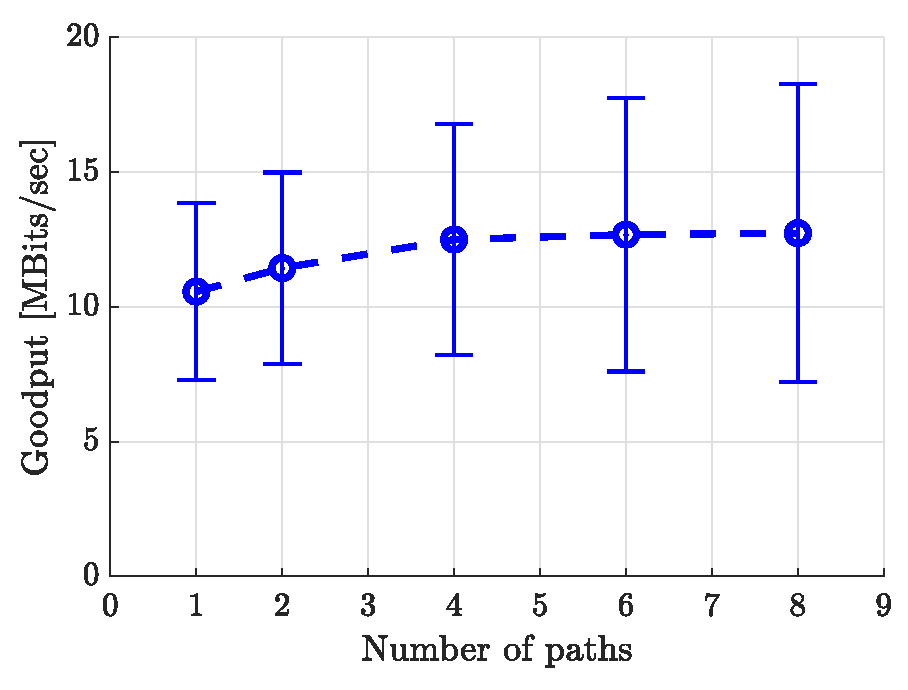
\includegraphics[scale=0.65]{../illustrations/performanceEvaluation/PerformanceWrtPathShortestpath.eps}  
		\caption[]{Plot of goodput depending on the number of paths used. An increasing number of paths leads to an increase in goodput. Path selection was done by minimizing the path length.}
		\label{fig:GoodputWrtToNOfPathsForShortestPath}
	\end{center}
\end{figure}

\subsection*{Influence of Path Selection}
\label{subsec:InfluencePathSelection}

Table \ref{tab:InfluenceOfPathSelection} shows the goodput obtained for the Shila-Measurement for all three path selection criteria. The chosen criterion does not influence the achieved performance. Reasons for this can be found in the topology of the SCIONLab network. Table \ref{tab:DiffFromOptimal}  shows the percentage deviation to the optimal value of the other metrics for each path selection algorithm. The optimal value of a certain metric corresponds hereby to the value obtained by optimization with the corresponding path selection algorithm. 

\begin{table}
	\begin{center}
		\ra{1.3}
		\begin{tabular}{lcccccc}\toprule
			Paths & MTU & Path length & Sharability \\\midrule
			1  & 10.37 {\small $\pm$ 3.17} & 10.57 {\small $\pm$ 3.28} & 10.34 {\small $\pm$ 3.24} \\
			2  & 11.67 {\small $\pm$ 3.72} & 11.44 {\small $\pm$ 3.55} & 11.26 {\small $\pm$ 4.18} \\
			4  & 12.55 {\small $\pm$ 4.34} & 12.5  {\small $\pm$ 4.29} & 12.09 {\small $\pm$ 4.64} \\
			6  & 12.45 {\small $\pm$ 5.32} & 12.68 {\small $\pm$ 5.08} & 12.75 {\small $\pm$ 5.37} \\
			8  & 12.63 {\small $\pm$ 5.37} & 12.74 {\small $\pm$ 5.53} & 12.46 {\small $\pm$ 5.72} \\\bottomrule
		\end{tabular}
		\caption{Listing of the achieved goodput in MBits/sec for different numbers of paths and path selection criteria. The algorithm used for path selection does not influence performance.}
		\label{tab:InfluenceOfPathSelection}
	\end{center}
\end{table}

\begin{table}
	\begin{center}
		\ra{1.3}
		\begin{tabular}{lccc}\toprule
			   			Paths & MTU & Path length & Sharability \\\midrule
			
			{\footnotesize Path Selection: }MTU			& & & \\
			1  	& - & 0 & 0    \\
			2  	& - & 0 & 0.72 {\small $\pm$ 0.21}  \\
			4  	& - & 0 & 0.34 {\small $\pm$ 0.16} \\
			6  	& - & 0 & 0.12 {\small $\pm$ 0.08} \\
			8  	& - & 0 & 0.06 {\small $\pm$ 0.06} \smallskip\\
			{\footnotesize Path Selection: }Path length  	& & & \\
			1  	& 0 & - & 0    \\
			2  	& 0 & - & 0.72 {\small $\pm$ 0.21} \\
			4  	& 0 & - & 0.34 {\small $\pm$ 0.16} \\
			6  	& 0 & - & 0.06 {\small $\pm$ 0.05} \\
			8 		& 0 & - & 0.05 {\small $\pm$ 0.05} \smallskip\\
			{\footnotesize Path Selection: }Sharability		& & & \\
			1  	& 0 & 0    & - \\
			2 	& 0 & 0.21 {\small $\pm$ 0.10}  & - \\
			4  	& 0 & 0.21 {\small $\pm$ 0.07} & - \\
			6  	& 0 & 0.16 {\small $\pm$ 0.07} & - \\
			8  	& 0 & 0.16 {\small $\pm$  0.07} & - \\\bottomrule
		\end{tabular}
		\caption{Percentage deviation to the optimal value of the other metrics for each path selection. Note that the Sharability for a single path is always zero. As an example of how to read the table: If the path selection is done using Sharability, the average length for two and four paths increases by 21\% compared to the optimal length. The optimal length is determined by the path selection using path length as an optimization criterion.}
		\label{tab:DiffFromOptimal}
	\end{center}
\end{table}

For all possible paths in the network, the same value for the MTU was obtained, irrespective of what metric for the selection was used. A possible positive effect of choosing paths with a higher MTU could therefore not be recognized at all. 

Comparing the average length of the paths, obtained when optimized for minimal path length and maximal MTU, no deviation was found. A possible negative effect of longer paths when using MTU instead of path length could therefore also not be observed. If we now bring the Sharability into play, we notice that an optimization by MTU or path length leads to a deterioration of the Sharability value. However, this has no negative impact on the goodput achieved. Such a negative effect could especially then be observed,  if bottlenecks in the network can be avoided by choosing the most different paths. If all shared links have sufficient capacity, this doesn't matter. We can therefore assume, that there were no capacity bottlenecks in the used links at the time the measurement was conducted. 

Concerning the Sharability values in Table \ref{tab:DiffFromOptimal}, two observations are noteworthy:

The values for the two path selection criteria MTU and Path length are almost identical. It is conceivable that the same selection resulted from both path selection procedures\footnote{Remember, the MTU is identical for all paths in the network.}. The path selection mechanism of Shila itself does not implement an explicit tiebreaker. However, the paths received from the SCION infrastructure may be already sorted by a criterion, in this case the length.

It is furthermore noticeable that the deterioration of Sharability is particularly marked when using just a few paths. This can be explained by the topology of the network. There are only a limited number of truly distinct paths between two endpoints available. As long as this number is not exhausted, the Sharability can be kept very small, but can also be large if a different metric for selection is chosen, hence the potential for deviation is large. Once all distinct paths are used up, additional paths have to include already used path segments. Hence the optimal value cannot be that small anymore, reducing the potential for deviation.

Using the Sharability as path selection criterion leads to an increase of the average path length between 15\% and 20\%. In the Shila-Measurement, this increase has no negative influence on the performance achieved. 

\subsection*{Comparison with QUIC over SCION}
\label{subsec:ComparisonWithQUIC}

Table \ref{tab:ComparisonWithQUIC} shows the values for goodput and throughput obtained from the Shila-Measurement and the Quic-Measurement. 

\subsubsection{Goodput}

Concerning goodput, QUIC over SCION outperforms Shila. Compared to MPTCP via SCION with a single path, QUIC achieves an average goodput that is more than three times better. With the use of eight paths for MPTCP via SCION the performance is still more than 2.5 times better. The data exchange with MPTCP via SCION means a detour for the data in both endpoints. The individual segments travel via a virtual interface to the kernel, back to the userland application Shila and from there through SCION and its networking stack. Once at the destination, the same procedure is repeated in reverse order. These additional distances inevitably lead to an increase of the Round-Trip-Time which has a negative effect on the achieved goodput.

\subsubsection{Throughput}

About a third of the total throughput of MPTCP over SCION is overhead. For QUIC over SCION it is only around 10\%, meaning that the latter approach performs better in this category as well. 

\begin{table}[H]
	\begin{center}
		\ra{1.3}
		\begin{tabular}{lcccc}\toprule
			Paths & \multicolumn{2}{c}{Shila-Measurement} & \multicolumn{2}{c}{Quic-Measurement}
			\\\cmidrule(lr){2-3}\cmidrule(lr){4-5}
			& \small{Goodput}  & {\small Throughput} & \small{Goodput}  & {\small Throughput} \\\midrule
			1  & 10.75 {\small $\pm$ 3.28} & 17.45 {\small $\pm$ 5.91}  & 33.31 {\small $\pm$ 3.28} & 36.82 {\small $\pm$ 3.62} \\
			8  & 12.74 {\small $\pm$ 5.53} & 19.37 {\small $\pm$ 8.36}  & - & -		 \\\bottomrule
		\end{tabular}
		\caption{Comparison of goodput and throughput in MBits/sec between the Shila-Measurement and Quic-Measurement. For Shila, path selection was done by minimizing the path length.}
		\label{tab:ComparisonWithQUIC}
	\end{center}
\end{table}

\section{Conclusion}

Based on the results obtained, the stated questions can be answered as followed:

{\small \begin{enumerate}
	\item How does the performance behave in relation to the number of paths used for a connection? \smallskip\\ \textbf{Increasing the number of paths leads to better performance. In the measurements conducted an increase in average goodput up to 20\% was observed.}
	\item How does the path selection influence performance?
	\smallskip\\ \textbf{Using different path selection algorithms does not influence performance. For the measurements carried out, none of the selection criteria was able to bypass a potential bottleneck in the network infrastructure and thus achieve better performance than the other criteria.}
	\item How well does Shila compare to QUIC over SCION?
	\smallskip\\ \textbf{QUIC over SCION outperforms MPTCP over SCION concerning goodput and overhead.}
\end{enumerate}}

Although the questions can be answered based on the taken measurements, a final answer to the performance of Shila should not be derived from them. Rather, these initial results should be used as the basis for further questions and improvements to Shila. In Chapter \ref{chap:FutureWork}, we discuss the questions that have emerged and possible improvements that can be addressed in future work.  